% Chapter 2

\chapter{Films polim\'ericos} % Main chapter title

\label{Chapter2} % For referencing the chapter elsewhere, use \ref{Chapter1}

%\section{papers of films}


Los hidrogeles consisten en una red de pol\'imeros entrecruzados altamente hidratados, generalmente biocompatibles, dependendiendo de su composici\'on qu\'imca. Estos materiales pueden parecerse al tejido biol\'ogico y dise\~narse para responder a cambios ambientales como variaciones de temperatura, pH, fuerza i\'onica y en la concentraci\'on de algunas biomol\'eculas. Como resultado, los hidrogeles polim\'ericos actualmente son candidatos prometedores para el desarrollo de una variedad de biomateriales con aplicaciones para biodetección [1,2], ingenier\'ia de tejidos [3,4], regeneraci\'on \'osea [5], materiales biomim\'eticos [6,7], administraci\'on de f\'armacos [8,9] y muchas otras aplicaciones biom\'edicas [10]. El ambiente acuoso dentro de los hidrogeles puede proteger a las prote\'inas de la desnaturalización y la agregaci\'on [11e13], mientras permanecen activas y estructuradas cuando se liberan de los hidrogeles [14]. En la administraci\'on oral de f\'armacos, los hidrogeles con respuesta de pH se han investigado en gran medida como veh\'iculos funcionales que pueden encapsular y administrar prote\'inas, evitando su degradaci\'on en el entorno gastrointestinal [15-17].


En este caitulo mostraremos un estudio  de estos sistemas polim\'ericos haciendo uso de de la te\'oria molecular mostrada en el capitulo anterior. 



\subsection{Caraterizaci\'on del sistema}
\textbf{pH} \\
Hidrogeles o films polim\'ericos compuestos por cadenas de poliacidos son sensibles a los cambios de pH. Esta respuesta se debe a la equilibrio qu\'imico de protonaci\'on/desprotonaci\'on de las unidades \'acidas que componen al red. 
Para enteneder el funcionamiento de esta respuesta vamos a recordar algunos conceptos sobre el comportamiento \'acido/base de moleculas bajo condiciones ideales. 
Estos conceptos nos serviran para entener el equilibrio que ocurre cuando se confinan los monomeros en una red polimerica.

Si consideramos una soluci\'on diluida de moleculas titulables, estas pueden exhibir dos estados posibles: protonado o desprotonado. El grado de disoción, $f_d$, nos proporciona la fraci\'on de moleculas que se encuentran en estado desprotonado:




\begin{equation}
    f_d = \frac{1}{1+10^{pk_a -pH}}
    \label{eq:diso}
\end{equation}
Para moleculas consideradas \'acidas el estado protonado es neutro y su estado desprotonado posee carga, por lo cual el grado de disociaci\'on nos indica el grado de carga de estas moleculas, $f_c$.
Para molecualas b\'asicas el grado de carga viene dado por: $f_c =1- f_d$.

En estas soluciones diluidad el grado de disociación $f_d$ (y el de carga $f_c$) son completamente determinados por el pH de la solución y el $pK_a$ intrinseco del par ácido/base. 
Cuando el pH =$pK_a$ la mitad de los grupos titulables se encuentran en disosiados ($f_d = 0.5$). Para valores de $\pm 1$ coresponden a estados con 90\% y 10\% de disociación respectivamente.
Es decir, cuando el pH aumenta alrededor del pKa, la transición del 10 al 90 \% de desprotonación ocurre dentro de dos unidades de pH de la solución ideal. A menudo, estas consideraciones de solución ideal se utilizan para estimar el grado de carga de las unidades ácidas dentro de la red de polímeros de hidrogel. Sin embargo, veremos a continuación que el confinamiento de estas unidades en una red polimérica modifica significativamente su comportamiento de protonación.

\textbf{Red polim\'erica} \\
En esta sección describiremos el comportamiento de carga de estos  hidrogeles sensibles al pH compuestos de cadenas de poliácido. A diferencia de las soluciones diluidas, las unidades ácidas en una red de polímeros experimentan repulsiones electrostáticas cuando estas se encuentran cargadas. Para reducir la fuerza de las repulsiones dentro de la red, estos grupos se disocian significativamente menos que en condiciones ideales.
En la figura \ref{fig:degree-film} ilustra este comportamiento y muestra el grado medio de carga de los segmentos de una película de hidrogel de ácido poli(metacrílico) (PMAA), que está en contacto con soluciones que tienen diferentes concentraciones de sal.
\begin{figure}
    \centering
    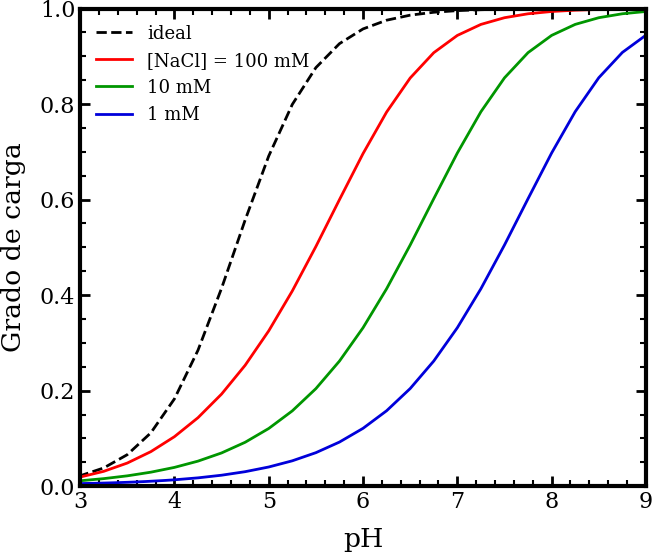
\includegraphics[width=0.9\textwidth]{Figures/graph-film/charge_degree-film.png}
    \caption{Grado de carga del gel como funci\'on del pH. Grado de carga para un monomero aislado en presentado en curva a rayas, se compara paa concentraciones de sal diferente, a mayor concentraci\'on salina m\'as nos acercamos al sistema ideal.}
    \label{fig:degree-film}
\end{figure}



A un pH dado, es significativamente menos probable que se cargue una unidad ácida de la red de lo que se espera según las consideraciones ideales. La concentración de sal de la solución resulta ser una variable crítica que modula este comportamiento de regulación de carga. A una salinidad relativamente alta, se encuentran concentraciones significativas de los contraiones dentro del hidrogel, lo que da como resultado el apantallamiento de interacciones electrostáticas, que volviendose de corto alcance. Esta apantallamiento de repulsiones dentro de la red permite que el polímero aumente su grado de carga para reducir la energía libre descripta por el equilibrio ácido-base de los segmentos de la cadena. El aumento en la salinidad genera una protonación que se aproxima al comportamiento ideal. En condiciones de baja salinidad, por otro lado, aumenta el costo entrópico de confinar iones dentro del hidrogel. Solo se encuentran los suficientes contraiones dentro de la red para neutralizar la carga eléctrica del polímero. Bajo tales condiciones, el efecto de apantallamiento de los iones de sal se debilita y las interacciones electrostáticas se vuelven efectivamente de mayor alcance. Como resultado, la red se carga menos para prevenir o reducir las repulsiones dentro de la red.

Otro aspecto a considerar es el pH local el cual es definido en la posición espacial \textbf{r}  utilizando la concentración local de protones:
\begin{equation}
    pH(r) = -\log_{10}([H^+](r))
    \label{eq:pH-local}
\end{equation}
Una baja disociación (un nivel de protonación alto) de las unidades ácidas del polímero puede explicarse en terminos del pH local dentro del material. Se define el $pH_{gel}$ como el promedio del pH local dentro del film. Resultados previos han mostrado que esta cantidad esta bien definida \addcite. En esta sección enfatizaremos la importancia de estos dos terminos $pH_{gel}$ y $pH(r)$ por la información que proveen: el estado de carga/protonación de las unidades titulables en la red polimérica. 

Haciendo uso de la eq. \ref{eq:diso} es posible calcular el grado de disoción de la estructura polimérica. El uso del $pH_{gel}$ es indispensable para cuanod el pH es distinto al  del seno de la solución \addcite. El mismo procedimiento se realiza para calcular el estado de protonación local de las unidades titulables de las especies que se adsorben en el film (ver figura \ref{fig:protein-charge}).

\begin{figure}
    \centering
    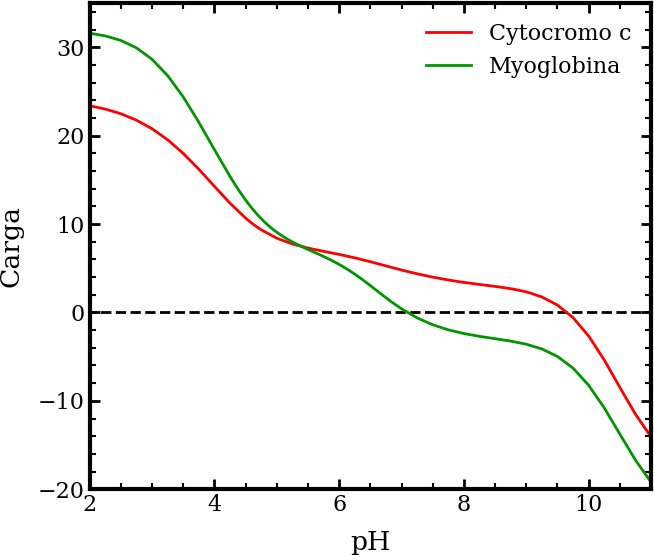
\includegraphics[width=0.9\textwidth]{Figures/graph-film/carga-proteinas.png}
    \caption{N\'umero de carga de las proteinas cytocromo c y myoglobina como  funci\'on del pH en el seno de la soluci\'on (bulk). La l\'inea a trazos muestra el cambio en el signo de la carga.}
    \label{fig:protein-charge}
\end{figure}



Sin embargo, aunque esto parece simplificar el problema de establecer la carga neta de cualquier especie dentro del material, incluida la red polimérica y las proteínas adsorbidas, determinar los cambios en el pH local tiene la misma complejidad que el problema original (es decir, determinar la carga de la la red). El pH local que se establece dentro del material, así como su valor en la interfaz entre el polímero y la solución acuosa, es el resultado de la compleja interacción entre la organización molecular, los equilibrios químicos y las interacciones físicas que determinan el equilibrio termodinámico a las condiciones impuestas externamente (pH, concentración de sal). Por ejemplo, la figura \ref{fig:pH-local} muestra el pH dentro de una película de hidrogel de PMAA como una función del pH  y la concentración de sal, calculado usando teor\'ia molecular.

\begin{figure}
    \centering
    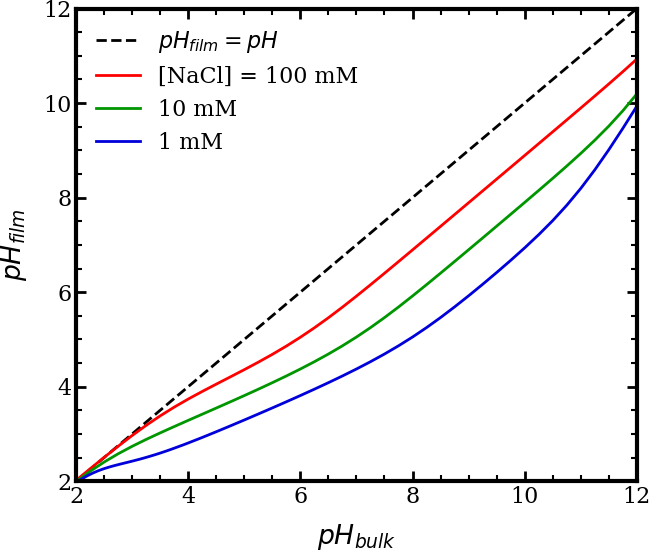
\includegraphics[width=0.9\textwidth]{Figures/graph-film/pH-local.png}
    \caption{pH local del gel como funci\'on del pH en el seno de la soluci\'on (bulk). Cada curva corresponde a una concentraci\'on de sal diferente.}
    \label{fig:pH-local}
\end{figure}

\subsection{Adsorci\'on}
Como se mencion\'o al incio de este capitulo... poder usar estos sistemas de hidrogeles como carries de adsrobatos de utilidad terap\'eutica.
Para ello nos valdremos de la teor\'ia molecular y haciendlo uso de ciertas prote\'inas modelo como lo son el cytocromo c y la myoglobina. estas dos presentan gran estabilidad en un amplio rango de pH y recientemente se ha  investigado la termodinámica  de su adsorci\'on en sistemas polim\'ericos similares. \addcite

Para cuantificar la cantidad de adsrobato adsrobido en el hidrogel utilizamos la expresi\'on:

\begin{align}
\Gamma = \int_V {dr(\rho(r) -\rho_{bulk}}  
\label{adsor}
\end{align}

en donde $\rho(r)$ y $\rho_{bulk}$ son las densidades del  locales y en el seno de la soluci\'on del adsorbato respectivamente, V es el volumen de la soluci\'on. 
Esta adsorción proporciona la masa  en un volumen particular por exceso de la contribución del bulk. En particular dentro del hidrogel, $\Gamma$ proporciona la cantidad de adsorbato en exceso dentro del material, recibiendo también contribuciones de la interfaz de solución de polímero.

Para estas proteínas, la adsorción es una función no monotónica del pH de la solución (ver Figura \ref{fig:ad-pro}). A pH bajo, estas proteínas tienen una carga alta y positiva, pero la red de poliácidos solo está débilmente ionizada (véanse las Figuras \ref{fig:degree-film} y \ref{fig:protein-charge}). A un pH suficientemente alto, por otro lado, el polímero está fuertemente cargado negativamente, pero las proteínas tienen una carga débilmente positiva o incluso negativa. Bajo tales condiciones (muy) ácidas o alcalinas, las interacciones electrostáticas son débilmente atractivas o repulsivas. No hay fuerza impulsora para la adsorción. A valores de pH intermedios, por el contrario, donde tanto la proteína como la red de poliácidos tienen cargas fuertes y opuestas, se produce una adsorción significativa con un máximo necesario en tales condiciones.

La adsorción de proteínas depende críticamente de la concentración de sal de la solución. Este comportamiento se ilustra en la figura \ref{fig:ad-pro} que muestra la adsorción de citocromo c  y mioglobina en una película de hidrogel de PMAA. La disminución de las concentraciones de sal mejora la adsorción y amplía el rango de pH de la adsorción. Por ejemplo, ambos paneles de la \ref{fig:ad-pro} muestran una disminución de aproximadamente un orden de magnitud en la adsorción cuando se comparan soluciones de NaCl 1 mM y 10 mM. El pH de máxima adsorción también depende de la salinidad de la solución. Este comportamiento es aún más interesante cuando se considera que una concentración de sal más baja conduce a una red con carga más débil, como describimos con anterioridad. En otras palabras, la red de polímero con carga más débil, a medida que disminuye la concentración de sal, más proteína es adsorbida. Esta última afirmación es cierta en las concentraciones de proteína ($10 \mu M$) y sal de la figura \ref{fig:ad-pro}, donde la adsorción solo modifica ligeramente el grado de carga de la red.

Esta dependencia de la adsorción de la concentración de sal tiene tres razones principales: en primer lugar, existe la protección de las atracciones electrostáticas de la red de proteínas por parte de los iones de sal. Cuanto menor sea la concentración de sal, más débil será la detección de las interacciones proteína-red, lo que mejora la adsorción. En segundo lugar, a medida que la concentración de sal disminuye, el pH dentro de las gotas de hidrogel (a un pH general dado). Esto implica que las proteínas adsorbidas tienen una carga más positiva tras la adsorción (a medida que disminuye ½NaCl?). En tercer lugar, la ganancia entrópica de la liberación de contraiones de la red de polímeros es mayor a medida que disminuye la concentración de sal, lo que también favorece la adsorción de proteínas.



\begin{figure}
    \centering
    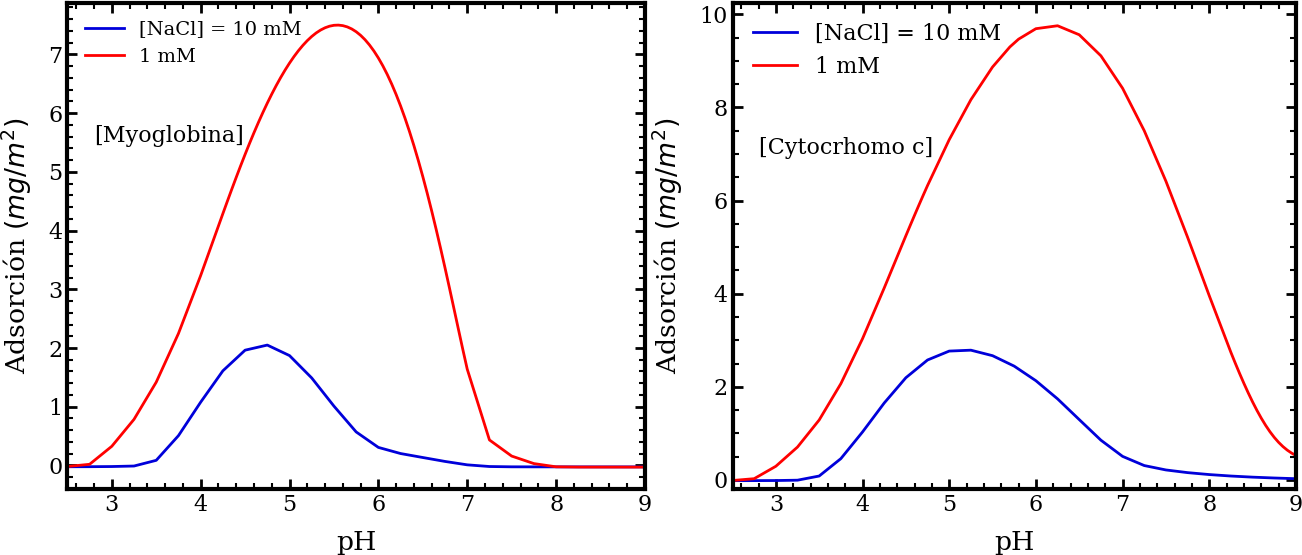
\includegraphics[width=0.99\textwidth]{Figures/graph-film/ad-proteins.png}
    \caption{Adsorci\'on de proteinas: cytocromo c y myoglobina en panel A y B respectivamente. La concentraci\'on de los adsorbatos es $10 \mu M$}
    \label{fig:ad-pro}
\end{figure}
